\documentclass[conference]{IEEEtran}
\IEEEoverridecommandlockouts
% The preceding line is only needed to identify funding in the first footnote. If that is unneeded, please comment it out.
\usepackage{comment}
\usepackage{subfigure}
\usepackage{multirow}
\usepackage{url}
\usepackage{cite}
\usepackage{flushend}
\usepackage{amsmath,amssymb,amsfonts}
\usepackage{algorithmic}
\usepackage{graphicx}
\usepackage{textcomp}
\usepackage{xcolor}
\def\BibTeX{{\rm B\kern-.05em{\sc i\kern-.025em b}\kern-.08em
    T\kern-.1667em\lower.7ex\hbox{E}\kern-.125emX}}
\begin{document}

\title{A Multi-Representation Ensemble Approach to Classifying Vocal Diseases}
\author{\IEEEauthorblockN{Mingxuan Ju, Zhengkai Jiang, Yufan Chen and Soumya Ray}
\IEEEauthorblockA{Department of Electrical Engineering and Computer Science, Case Western Reserve University, Cleveland, OH 44106}
\IEEEauthorblockA{Email: {\{mxj255, zxj89, yxc775, sray\}@case.edu}}
}
\maketitle
\begin{abstract}
The goal of the IEEE 2018 FEMH Voice Data Challenge was to develop an effective algorithmic approach to classifying voice samples as normal or pathological, and further subdivide the pathological samples into three types. We adopted a multi-representation ensemble approach to the task. We designed a pipeline with three classification stages, where each stage used a combination of supervised, semi-supervised and multiple-instance learners. This approach was able to achieve a sensitivity of 89\% and specificity of 76\% in classifying normal from pathological samples and an unweighted average recall (UAR) of 60.67\% in subclassifying pathological samples into three types.
\end{abstract}
%\tableofcontents

\section{Introduction and Background}
The goal of the IEEE 2018 FEMH Voice Data Challenge was to develop an effective algorithmic approach to classifying voice samples as normal or pathological, and further subdivide the pathological samples into three types: vocal palsy, phonotrauma or neoplasm. As noted by the challenge organizers, voice disorders can severely affect quality of life, since humans primarily rely on speech for communication. At the same time, diagnoses of vocal disorders depend on larygeal endoscopy, which requires human expertise and specialized equipment. Thus there is a need for algorithms that could for example be used to triage cases to focus scarce resources.

The task of differentiating normal from pathological voice samples has been investigated in previous work, with a summary of previous approaches in~\cite{b9}. Among these approaches are artificial neural network with Mel-Frequency-Cepstral-Coefficients(MFCC), feature vectors from multiple frames that collectively represent the power spectrum of a sample~\cite{b5}. Others have used wavelet transform with support vector machines (SVMs)~\cite{b4}. Recently a deep neural network~\cite{b9} has been used by dividing the raw waveform into multiple segments and extracting normalized MFCC features from them.

A concern with some previous work is that they use a very old database of voice disorders from Massachusetts Eye and Ear Infirmary (MEEI), collected in 1994. It is not clear how well methods developed on this database might generalize to new data, for example because the recordings occurred in a well controlled environment. Indeed, recent previous work shows that learning algorithms can typically achieve a very high accuracy on data from this database. A contribution of the challenge organizers was to create a new dataset to see how well the MEEI results generalized to other cases. As the organizers note~\cite{}, the released dataset contains voice samples obtained from a voice clinic in the Far Eastern Memorial Hospital (FEMH). The training dataset includes 50 normal voice samples and 150 samples of common voice disorders, including vocal nodules, polyps, and cysts; laryngeal neoplasm; and unilateral vocal paralysis. The labels of the training dataset includes gender, age, whether the speaker is health or not, and the corresponding voice diseases. There are 400 testing samples without any labels for performance evaluation. All FEMH voice samples are a 3 second sustained vowel sound /a:/, which were recorded at a comfortable level of loudness, with a microphone-to-mouth distance of approximately $15-20$ cm, using a high-quality microphone (Model: SM58, SHURE) with a digital amplifier (Model: X2u, SHURE). X\% of the samples were male and the rest female. The sampling rate was 44100 Hz with a $16-$bit resolution, and data were saved in an uncompressed .wav format. Although we were allowed to use the MEEI database to train our models, we elected not to do so.


%\subsection{Background and Related work:}
	Vocal classification is perceived as one of the challenging tasks in medical field. Many researchers did meaningful work on designing optimal classifiers which can help diagnose vocal diseases from patient's voice record. Some vocal diseases such as neoplasm are notoriously hard to distinguish solely by listening due to noise and subtlety of symptom. 
	Most researchers designed optimal algorithm and ways to extract features in audio classification.
	Vahid Majidnezhad tried artificial neural network with Mel-Frequency-Cepstral-Coefficients as feature vectors to achieve optimal result on vocal pathology classfication\cite{b5}. P. Kukharchik also used wavelet transform with support vector machine to optimize classifiers' performance\cite{b4}. Shih-Hau Fang's team also use deep neural network to train classifier by diving the raw waveform into multiple segments, extract normalized MFCC features from them and feeding them into neural network. They also get optimal result from this\cite{b9}.
	However, there are not any researcher who has explored the multiple-ensemble classification by dividing mul-class classification into multiple binary classification in vocal pathology classification, which is what this paper will explore on. 

	  % Yufan Chen
\section{System Description}
\def\hyp{\mathbf{w}}
\def\boldxi{\mbox{\boldmath$\xi$}}
\def\smallboldxi{\mbox{\boldmath\scriptsize{$\xi$}}}

The challenge as described was clearly separated into two phases. First, we needed to classify the given audio samples into normal or pathological. Then, the pathological samples were to be classified into one of three kinds: vocal palsy, phonotrauma or neoplasm. Upon an initial inspection and analysis of the data, we observed that vocal palsy seemed the easiest to tell apart from normal by listening to the samples. Therefore, we decided upon a pipeline based approach (Figure~\ref{fig:}). In the pipeline, after preprocessing, we first check if a new sample is normal or not. If a sample is classified as abnormal, it is sent to the second stage, where we decide if it is a sample corresponding to vocal palsy. If this stage returns negative, we proceed to the final stage where the sample is assigned a label corresponding to either phonotrauma or neoplasm. An advantage of this approach instead of a simple multiclass approach is that, by eliminating many samples for consideration by the later stages of the pipeline, we may hope to improve accuracy over classifying everything at once. On the other hand, this approach leaves the most ``confusing" examples for the last classifier, and since we do not have the option of returning an ``I don't know" label, it may be that our phonotrauma vs neoplasm classifier could have a lower accuracy.

The next consideration was the algorithm to use as a classifier in each stage. Recent machine learning systems and competitions~\cite{} have shown that ensemble approaches are often the best at solving complex problems. This is because typically, a diverse ensemble of classifiers can have elements that each focus on a different aspect of the problem so that when results are combined, the entire system does well. We also chose to follow this principle in designing our classifiers. 

The next question to answer was how to design our ensemble. Rather than going with an off-the-shelf approach, we chose to build an ensemble that was customized to the problem. In particular, we decided to select our ensemble classifiers from three different paradigms: supervised, semi-supervised and multiple-instance learning. The choice of supervised learners was obvious since this task was set up as a batch supervised problem. However, the challenge organizers also provided an unlabeled test set, which was twice the size of the training set. We realized that this could be used as additional information during training. This was especially the case since (as we describe later) we found that doing well on the training set  using cross validation did not guarantee good results on the test set. Therefore we added a semi-supervised component~\cite{} which could use the unlabeled test data during learning. Finally, the task as described can also be formulated as a multiple-instance (MI) problem. In MI learning, an example is described by a {\em set} (called a bag) of feature vectors. If an example is labeled positive, at least one instance in the bag is positive; if it is negative, all instances are negative. The task is to learn a bag or instance classifier from such data. In the given task, suppose we partition the given audio samples into windows of some time intervals. Then, we argue that if a voice sample exhibits vocal palsy, or phonotrauma, or neoplasm, {\em there must be at least one window} which contains a signal of that abnormality. Conversely, if a sample is normal, no window contains any abnormality. Therefore this maps well onto the MI learning task. This approach may perform better than analyzing the entire sample because it is possible for most of a sample to be ``normal" even though the patient has a disease. ``Focusing" on a specific fragment of a sample may therefore be better than considering the sample as a whole.

We instantiated the three paradigms as follows.  For supervised learning we used a support vector machine~\cite{} (SVM). SVMs are well-known classification algorithms that have demonstrated excellent performance in many practical applications. They were also evaluated in prior work on this task~\cite{}. An SVM learns a linear classifier which maximizes the margin by solving the quadratic program (QP): $\underset{\hyp,b,\smallboldxi}{\min}\tfrac{1}{2}\left\lVert  \hyp\right\rVert^2 + C\sum_{i}\xi_i$, such that $y_i\left(\left<\hyp,\phi(x_i)\right> + b\right) \ge 1 - \xi_i$ and $\boldxi \ge 0$. The slack variables $\boldxi=\{\xi_i\}$ allow for
some misclassification of points, and the objective function seeks to minimize
this error on the training data. $C$ is a parameter that trades off  error and
regularization. The dual form of the QP shows that the
separator $\mathbf{w}, b$ can written as a dot product $\langle
\phi(x),\phi(y)\rangle$, so we can use a kernel function $k(x,y)$ to
implicitly represent the feature space $\phi$. We use linear and radial basis function (RBF) kernels in our system. The linear kernel is simply $k(x_i,x_j)= x_i\cdot x_j$ while the RBF kernel is defined by $k(x_i,x_j) = exp(-\gamma||x_i - x_j ||^2)$\cite{b12}.

For semi-supervised learning, we used two approaches: label propagation~\cite{} and a transductive SVM~\cite{}. Label propagation (LP) assumes a set of labeled and unlabeled points that are arranged as a graph. Edges on the graph are weighted by similarity. LP computes a real-valued function $f: V\rightarrow R$ on the vertices of the graph that minimizes an energy function $E(f)=\sum_{i,j}w_{ij}(f(i)-f(j))^2$, where $w_{ij}$ is the weight on the edge $(i,j)$. The solution can be obtained in closed form and produces a labeling of all unlabeled points in the set of examples. Transductive SVMs extend the basic SVM QP by adding constraints for all unlabeled points, while leaving their labels unknown to be set by the optimizer: $\underset{\hyp,b,\smallboldxi,y_u}{\min}\tfrac{1}{2}\left\lVert  \hyp\right\rVert^2 + C\sum_{i}\xi_i+ \hat{C}\sum_{u}\xi_u$, such that $y_i\left(\left<\hyp,\phi(x_i)\right> + b\right) \ge 1 - \xi_i$, $y_u\left(\left<\hyp,\phi(x_u)\right> + b\right) \ge 1 - \xi_u$, $y_u \in \{-1,+1\}$, $\boldxi \ge 0$. Here the variables indexed by $u$ correspond to the unlabeled set. This is a mixed integer programming problem which is NP-hard to solve in the worst case. However, heuristic approaches exist that have been shown to perform well~\cite{}.

For multiple-instance learning, we use multiple-instance logistic regression (MI/LR)~\cite{}. This algorithm estimates the probability $\Pr(y_i=1|B_i)$ for a bag $B_i$ from the instances $\{B_{i1},B_{i2},... ,B_{in}\}$ in it. To do this it uses logistic regression to estimate conditional probabilities for each instance,
and softmax to combine these to obtain the conditional
probabilities for each bag:
\begin{eqnarray}
S_{ij}=\Pr(y_{ij}=1|B_{ij})=\frac{1}{1+e^{-({\bf w}\cdot
    B_{ij}+b)}} \nonumber\\
\Pr(y_i=1|B_i)=\mbox{softmax}_\alpha(S_{i1},\ldots,S_{in}) \nonumber
\end{eqnarray}
Note that here, the softmax function encodes the MI assumption that labels a bag positive if at least one instance in it is positive.

To combine the output of these ensembles, we use the following strategy. Initial testing showed that MI/LR had a very high cross-validated area under the ROC graph (AUC) score, sometimes exceeding $0.9$. Therefore we combine the outputs of the predictors as follows: a sample is labeled positive if MI/LR's conditional probability exceeds $0.85$, and negative if the conditional probability is below $0.15$. If the conditional probability lies between these values, then we return a majority vote of the elements of the ensemble.

We also considered stratifying our models based on gender. Some prior work suggests that features may have different distributions in men and women and so there may be value in training separate models. However, we had limited training data and further subdividing it to train gender-specific models did not seem feasible.

\subsection{Data Preprocessing, Implementation and Validation}
A check on the data showed that there was a period of silence at the beginning of most audio files. We removed these parts by calculating the average loudness of each audio file, and removing the prefix of the file that was below  30\% of the average loudness. No other preprocessing was performed on the given data.

All of our algorithms and features were implemented in Python. We used the libraries....[WRITE THIS WITH CITATIONS]. 

Our internal experimentation on the training sets with the supervised and multiple-instance algorithms were performed using 5-fold cross validation. We used these experiments to pick the supervised algorithms to use in our ensemble. We also tried using other approaches such as decision trees and random forests, but they did not perform well on our data.

The SVM classifiers have hyperparameters that need to be tuned. Since the size of training set is getting smaller and smaller as we propagate through the pipeline, in order to tune hyperparameters for all three ensembles, we use the same hyperparameter value obtained in the first ensemble (normal/pathological). Tuning is done through internal cross validation for the hyperparameters $C$ and $\gamma$ independently. The tuned values are 10 for C, and 0.01 for $\gamma$. We also modify the class weight with respect to the proportion of class in the objective function of the SVM in order to correct for class imbalance, since (for example) in the initial task there are only 50 normal samples and 150 pathological cases. This class imbalance parameter is also tuned via the same procedure. 

% \subsection{Validation Method:}
% Before mentioning detailed structure and algorithm we have attempted, I want to point out that we measure accuracy using stratified 10-fold cross validation(CV). Any classifier's accuracy is the weighted average accuracy of numbers we get from 10 folds.  \\
% \indent However, for transductive learning algorithm such as Transductive Support Vector Machine or Label Propagation, we could not do cross validation since there is no validation set for transductive learning. Accuracy we have on those algorithms is the accuracy on whole training set, in other word, the rate of convergence. 
% % \subsection{Attempted Algorithms:}
% Tree-Based Algorithms:
% \begin{itemize}
	% \item Decision Tree:\\
	% Utilizing tree structures, decision tree algorithm calculates entropy of each feature and splits node based on the rank of features with respect to their entropies. Probably due to the fact that different classes are representative in different features and skewed class distribution, a single decision tree could not solve this learning problem and we only get 62\% accuracy on CV.\\
	% \item Random Forest:\\
	% Instead of having a single tree structure, Random Forest fits a number of decision tree classifiers on various sub-samples of the dataset.\cite{b7} Using Random Forest classifier, we get 89\% accuracy on CV. But even with such high accuracy, Random Forest performs poorly on test set according to the feedback from oracle. We analyze that the differences on performance between training set and testing set probably result from skewed data distribution and over-fitting. \\
% \end{itemize}

% \indent Based on cross validation results on experiments we have done, it seems like tree-based algorithm generally is inappropriate for this learning task. \\

% Support Vector Machines(SVMs):\\
% \begin{itemize}
	% \item Linear SVM:\\
	% Based on the features' distribution of each training example, SVM differentiates classes by building a hyperplane that maximizes the margin between classes. And for Linear SVM, the decision boundary is a linear function. The kernel of Linear SVM is simply the hyperplane function $K(x_i,x_j) = \phi(x_i)*\phi(x_j) = (x_i*x_j)^2$, and in order to maximize the margin between plus-plane and minus-plane to get best generalization, SVM minimized the norm of parameter $w$\cite{b12}. After tuning loss penalty and class weight, we get 89\% accuracy on CV and a relatively reasonable classification on test set according to the feedback from oracle.\\
	% \item SVM with Radial Basis Function kernel(SVM-RBF):\\
	% Pretty similar to Linear SVM, SVM-RBF differs by the non-linear kernel function. The SVM-RBF formulation differs from Linear SVM by having an non-linear kernel function, which could be represented as $K(x_i,x_j) = exp(-\gamma||x_i - x_j ||^2)$\cite{b12}. After having a reasonable result from Linear SVM, we were excited on trying SVM-RBF(with tuned loss penalty and gamma). It ends up having 89\% on CV and similar test set performance. However in the late phase, we discarded SVM-RBF because with the number of features we have, it is possible that a non-linear kernel function over-fits. \\
% \end{itemize}

% Transductive Learning Algorithms:\newline\\
% \indent Noticing that size of test set is twice size of training set, in order to get better generalization, we want to utilize test set and attempted several transductive learning algorithms. \\
% \begin{itemize}
	% \item Label Propagation:\\
	% Identifying the test example's closest training set neighbor, Label Propagation assigns the same label that neighbor has to the test example. The edge between any two examples i and j, is weighted to be so that the closer the nodes are in local Euclidean distance, the larger the weight $w_{ij}$, the weight is controlled by a parameter $\theta$ :  $w_{ij} = exp (\frac{(d_{ij}^2)}{\theta^2}) = exp (-\frac{\sum_{d = 1}^{D} (x_{id} - x_{jd})^2}{\theta^2} )$. \cite{b13}Without CV on this algorithm, we compare the number of assigned labels of each class to that from SVMs. From Label Propagation, we get 69 Normals, 107 Vocal Palsys and 171 Phonotraumas. From Linear SVM, we get 65 Normals, 79 Vocal Palsys and 167 Phonotraumas.\\
	% \item Transductive Support Vector Machine(TSVM):\\
	% This is a SVM-RBF based classifier with test set regulating the range of how far away the hyperplane can extends. The kernel function of SVM-RBF is represented as $K(x_i,x_j) = exp(-\frac{||x_i - x_j ||^2}{2\gamma^2})$\cite{b14}. Although in test set, TSVM overcalls a great number of Normal, it could give us a board view of all 'Normal-ish' examples, and later on we could limit our focus on this specific set of Normals. \\
% \end{itemize}

% Multiple Instance Learning Regression(MILR):\\
% \begin{itemize}
	% \item 
	% Instead of receiving a set of instances which are individually labeled, the learner receives a set of labeled bags, each containing many instances. In the simple case of multiple-instance binary classification, a bag may be labeled negative if all the instances in it are negative. On the other hand, a bag is labeled positive if there is at least one instance in it which is positive. \cite{b10} Although MILR undercalls Normal, having super high Area under ROC Curve(AUC) 0.92, MILR could work as an oracle and we only focus on test examples labeled with confidence higher than 85\%.\\
% \end{itemize}
% \subsection{Final Architecture Overview:}
	% Our whole model-building infrastructure is based on scikit-learn\cite{b7}\cite{b8}. \\
	% \indent We tried Support Vector Machine, Boosting, Random Forest, Extratrees, Multiple Instance Learning, Label Propagation. After few experiments, it seemed like tree algorithms performed poorly on this task and we finalized our focus on SVM, Label Propagation, SVM-RBF and MILR with pipeline. Any single classifier undercalled Normal and Neoplasm patients, which we think is resulted from different class distributions between training and testing set. \\
% \indent So, we converted this relatively complex learning task into three less complicated tasks: Normal vs. Pathological, Vocal vs. Rest of Diseases, and Phonotrauma vs. Neoplasm, with each learning task having ensemble consisted of 4 classifiers.[Fig. 1] The reason why we design the pipeline this way is based on the difficulty of classification according to our perception. (From easiest Normal vs. Pathological to hardest Phonotrauma vs. Neoplasm)\\

	\begin{figure}[!htbp]
		\begin{center}
			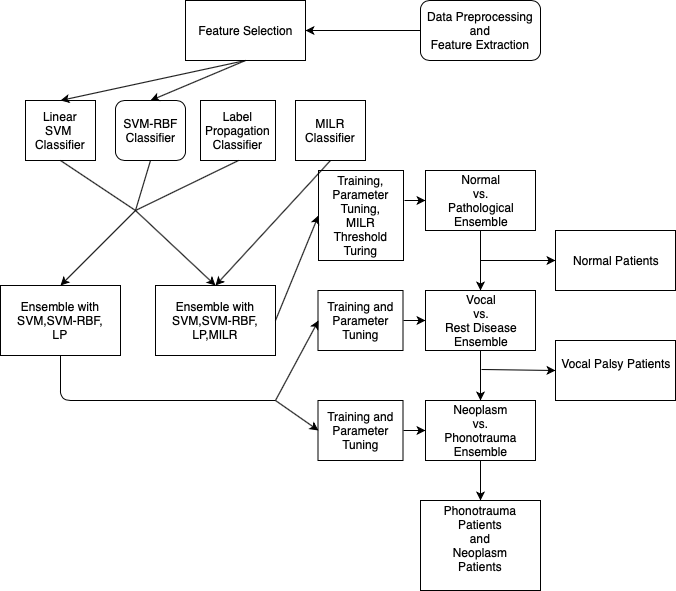
\includegraphics[scale=0.35]{Diagram_3.png}
		\end{center}
		\caption{The Process of Classifying, including classifier training, ensemble structures and pipeline implementation}
	\end{figure}

% \subsection{Feature Selection:}
% Due to the fact that the size of our training set is relatively small, in case of over-fitting, for each classifier we select 50\% best features, with respect to entropy, according to Renyi's feature selection.\cite{b14} However, it seems like feature selection jeopardizes the performance of transductive learning. So we only utilize feature selection on SVM and SVM-RBF.

% \subsection{Hyper Parameter Tuning:}
% Since the size of training set is getting smaller and smaller as we propagate through the pipeline, in order to get trustworthy accuracy to tune parameter for SVC, for all three ensembles, we use the same parameter tuned in the first ensemble. The process is pretty straightforward; we simply set up two loops, one of which for C and one of which for gamma. The tuned parameters are 10 for C, and 0.01 for gamma. Also due to the skewed distribution in training set, we modify the class weight with respect to the proportion of class. 


   % Mingxuan Ju
\section{Feature Extraction}
We now describe the feature set that we extract from the given audio files. These features are used with the classifiers above. Many of these features are widely used in machine learning for audio classification. The last feature, ``Number of Amplitude Peaks and Vallies" is created by us. The features are:
\begin{enumerate}
	\item Zero Crossing Rate (ZCR):\\
	The rate of sign-changes of the signal during the duration of a particular frame~\cite{b1}: $ZCR=\frac{1}{T-1}\sum_{t = 1}^{T - 1}I_{R<0}$, where $R = (s_t * s_{t-1})$ and $s$ is signal with length $T$.
	\item Energy:\\
	The sum of squares of the signal values, normalized by the respective frame length~\cite{b2}: $Energy = \sum_{i = 1}^{N} \frac{s_i^2}{|s_i|} $, where $N$ is the total number of blocks of signals and, $s_i$ is the signal in frame $i$.
	\item Entropy of Energy (EE):\\
	The entropy of sub-frames' normalized energies. It can be interpreted as a measure of abrupt changes.~\cite{b2} Setting number of sub-frames $n$ to $10$, we calculate EE by: EE = $\frac{(\frac{L}{n})^2}{Eol +\epsilon} \log_{2}({(\frac{(\frac{L}{n})^2}{Eol +eps} + eps})$, where $L$ is the length of audio signal, $\epsilon$ is the learning rate and $Eol$ is the total energy of this signal.
	\item Spectral Centroid (SC):\\
	It indicates where the "center of mass" of the spectrum is located. Perceptually, it has a robust connection with the impression of "brightness" of a sound~\cite{b3}:  $SC = \frac{\sum_{n = 0}^{N - 1} f(n)x(n)}{\sum_{n = 0}^{N - 1} x(n)}$, where $f(n)$ is the frequency of current bin and $x(n)$ is weighted frequency value.
	\item Spectral Energy (SE):\\
	Entropy of the normalized spectral energies for a set of sub-frames.~\cite{b3}: $SE = \sum_{i = 1}^{N} \frac{1}{N} |x(s_i)|^2$, where $x(s_i)$ is the average amplitude of sub-frame $s_i$.\\
	\item Spectral Spread (SS):\\
	The second central moment of the spectrum~\cite{b3}:  SS = $\sqrt{\frac{\sum_{k = 0}^{\frac{N}{2}} (f(k)-SC)^2 |x(k)|^2}{\sum_{k = 0}^{\frac{N}{2}} |x(k)|^2 }}$, where f(k) is the frequency at k, N is the total length of the frame and x(k) os weighted frequency value \\
	\item Spectral Entropy:\\
	Entropy of the normalized spectral energies for a set of sub-frames\cite{b3}: $SpEn = -\sum_{i = 1}^{n} \frac{\frac{1}{N} |x(s_i)|^2}{\sum_{i}^{}\frac{1}{N} |x(s_i)|^2} \ln\frac{\frac{1}{N} |x(s_i)|^2}{\sum_{i}^{}\frac{1}{N} |x(s_i)|^2}$.
	\item Spectral Flux:\\
	The squared difference between the normalized magnitudes of the spectra of the two successive frames.~\cite{b3} 
	\item Spectral Rolloff:\\
	The frequency below which 90\% of the magnitude distribution of the spectrum is concentrated~\cite{b3}: $SpRo = \arg \min \sum_{i = 1}^{f_c} m_i \geq \sum_{i = 1}^{N}0.9 m_i$, where $f_c$ is the rolloff frequency and $m_i$ is the magnitude of the $i^{th}$ frequency component of the spectrum. 
	\item Mel Frequency Cepstral Coefficients(MFCCs):\\
	Mel Frequency Cepstral Coefficients form a cepstral representation where the frequency bands are not linear but distributed according to the mel-scale.~\cite{b4} A more detailed description of MFCC can be found in~\cite{b9}.
	\item Chroma Vector:\\
	A 12-element representation of the spectral energy where the bins represent the 12 equal-tempered pitch classes of western-type music (semitone spacing).\cite{b5} We calculate this by detecting the tone height and chroma of certain segment, and assign each element the vector it falls into.
	\item Chroma Deviation:\\
	The standard deviation of the 12 chroma coefficients.~\cite{b5}
	\item Number of Amplitude Vally and Peak:\\
	The number of amplitude peaks and vallies. We extract this feature by counting the number of frames where its amplitude derivative is 0. %The mathematical description of this feature is : $ \sum_{t = 1}^{N-1}  I_{dR=0}$, where dR is the derivative of amplitude curve, and N is the total length of this frame.\\
\end{enumerate}
Because we had a very small training set, for the supervised learning algorithms, overfitting was a concern especially later in the pipeline where there were fewer training examples. To reduce this effect, we used mutual information based feature selection~\cite{b25} for the SVMs (linear and RBF) and trained these models on 50\% of the features.

First 13 features are widely used in the field of machine learning for audio classification\cite{b26}\cite{b27}. We utilize an existing library\cite{b6} that implements first those features. The last feature Local Amplitude Minimum is introduced by us to help classifiers distinguishing normal audio and abnormal audio, which turns out to be extremely efficient.
\section{Results \& Discussion}


We have several different kinds of models including TSVM, SVM, Label Propagation and MILR in our ensemble. 

Some of these works well such as Label Propagation, it is able to detect 69 normal cases, but the MILR is capturing far fewer normal cases. However, there is a very high Area under ROC graph for MILR, 0.96. It seems that it is difficult to detect the normal cases. For TSVM, it is overcalling a lot of normal cases with the default 50\% confidence threshold, which have the opposite the problem compared with MILR. So we think that there might be some mismatches between the testing examples and training examples, probably there are some features that are not included in the training examples but appeared in the testing files. It is very obvious to see that the UAR for cross validation of SVM is 76.40\% and the UAR for test cases is only 64.77\%. So we have to change the confidence level in order to get a closer result.

We are able to detect the normal examples with 79.5\% in the cross validation for SVM, [number] \% for the MILR, but the actual result for the test cases is 60.0\%. We can see from Table 1. that there are 20\% difference between the two results. Since the other two methods are Label Propagation and TSVM, which are not able to do the cross validation, we can only analyze the SVM and MILR.


\begin{table*}[!htbp]
	\caption{CROSS VALIDATION AND ACTUAL RESULT}
	\begin{center}
		\begin{tabular}{|c|c|c|c|c|c|}
			\hline
			 & SVM CV & SVM-RBF CV & MILR CV & with TSVM & with SVM-RBF \\
			\hline
			Sensitivity$^{\mathrm{a}}$  & 88.8\%& 92.1\% & 53.3\% & 82.2 \% & 89.4\% \\
			\hline
			Specificity & 79.5\% & 52.0\%& 86.0\%& 60.0\% & 76.0 \% \\
			\hline
			Volcal palsy recall & 81.0\% &76.0\%& 30.0\% & N/A & N/A \\
			\hline
			Phonotrauma recall & 61.0\% &69.6\%&& N/A& N/A\\
			\hline
			Neoplasm recall & 81.1\% & 72.0\%&& N/A& N/A \\
			\hline
			UAR & 76.40\% &72.53\% & & 64.77\% & 60.67\%\\
			\hline
			\multicolumn{4}{l}{$^{\mathrm{a}}$ Number of correctly predicted pathological / total pathological}
		\end{tabular}
		\label{tab2}
	\end{center}
\end{table*}

\begin{table*}[!htbp]
	\caption{NUMBER OF NORMAL EXAMPLES PREDICTED IN TEST CASES}
	\begin{center}
		\begin{tabular}{|c|c|}
			\hline
			& Number of Normal \\
			\hline
			SVM & 56\\
			\hline
			SVM-With Feature Selection & 65\\
			\hline
			SVM-RBF & 84 \\
			\hline
			MILR & 257 \\
			\hline
			Label Propagation & 69 \\
			\hline
			TSVM & 261 \\
			\hline
			Ensemble with TSVM & 93\\
			\hline
			Ensemble with SVM-RBF & 74\\
			\hline
			Actual results& 122 \\
			\hline
		\end{tabular}
		\label{tab2}
	\end{center}
\end{table*}

Then, we tried another ensemble without the TSVM. We suspect that the there are problems caused by the over calling of normal by it. We changed the TSVM with the SVM-RBF. Then, we see an increase in both the sensitivity and specificity but the UAR decreased. From Table 1, We see that the Sensitivity increased by 7.2\% and Specificity increased by 16.0\%, though the Specificity of SVM-RBF is low, the other methods in the ensemble are able to catch those normal cases. However, there is a 4\% decrease in UAR score. We think that the SVM-RBF works better for distinguishing normal examples from pathological examples but the TSVM might work better for classification the different kinds of diseases. One possible reason might be that the two diseases Phonotrauma and Neoplasm are very close and hard to distinguish for SVM-RBF, we can see from Table 1, that the SVM-RBF only have around 70 \% of recall for both classes.
 
  % Zhengkai Jiang
\section{Conclusion}



\begin{thebibliography}{00}
	
\bibitem{b1}
 Gouyon F., Pachet F., Delerue O. (2000),On the Use of Zero-crossing Rate for an Application of Classification of Percussive Sounds, in Proceedings of the COST G-6 Conference on Digital Audio Effects (DAFX-00 - DAFX-06), Verona, Italy, December 7–9, 2000. Accessed 26 April 2011.

\bibitem{b2}
Müller, G., Möser, M. (2012). Handbook of Engineering Acoustics. Springer. p. 7. ISBN 9783540694601.

\bibitem{b3}
Grey, J. M., Gordon, J. W., 1978. Perceptual effects of spectral modifications on musical timbres. Journal of the Acoustical Society of America 63 (5), 1493–1500, doi:10.1121/1.381843

\bibitem{b4}
Beigi, Homayoon (2011). Fundamentals of Speaker Recognition. Berlin: Springer-Verlag. ISBN 978-0-387-77591-3.

\bibitem{b5}
Müller, Meinard (2015). Fundamentals of Music Processing. Springer. doi:10.1007/978-3-319-21945-5. ISBN 978-3-319-21944-8.

\bibitem{b6}
T. Giannakopoulos., pyAudioAnalysis: An Open-Source Python Library for Audio Signal Analysis, PloS One, 10, pp. 12, 2015

\bibitem{b7} 
Fabian Pedregosa, Gaël Varoquaux, Alexandre Gramfort, Vincent Michel, Bertrand Thirion, Olivier Grisel, Mathieu Blondel, Peter Prettenhofer, Ron Weiss, Vincent Dubourg, Jake Vanderplas, Alexandre Passos, David Cournapeau, Matthieu Brucher, Matthieu Perrot, Édouard Duchesnay, Scikit-learn: Machine Learning in Python

\bibitem{b8} 
Lars Buitinck1, Gilles Louppe2, Mathieu Blondel3, Fabian Pedregosa4, Andreas C. Muller5, Olivier Grisel6, Vlad Niculae7, Peter Prettenhofer8, Alexandre Gramfort4,9, Jaques Grobler4, Robert Layton10, Jake Vanderplas11, Arnaud Joly2, Brian Holt12, and Ga''el Varoquaux4, API design for machine learning software: experiences from the scikit-learn project

\bibitem{b4}
P. Kukharchik, D. Martynov, I. Kheidorov and O. Kotov, "Vocal fold pathology detection using modified wavelet-like features and support vector machines," 2007 15th European Signal Processing Conference, Poznan, 2007, pp. 2214-2218.

\bibitem{b5}
Majidnezhad, V. and Kheidorov, I., 2013. An ANN-based method for detecting vocal fold pathology. arXiv preprint arXiv:1302.1772.

\bibitem{b9}
Shih-Hau Fang, Yu Tsao, Min-Jing Hsiao, Ji-Ying Chen, Ying-Hui Lai, Feng-Chuan Lin, Chi-Te Wang,
Detection of Pathological Voice Using Cepstrum Vectors: A Deep Learning Approach,
Journal of Voice, 2018,
\bibitem{b10}
S. Ray \& M. Craven (2005).
Supervised versus Multiple-Instance Learning: An Empirical Comparison.
Appears in the Proceedings of the 22nd International Conference on Machine Learning, Bonn, Germany.
\bibitem{b11}
Far Eastern Memorial Hospital, FEMH, https://www.femh.org.tw
\bibitem{b12}
Cortes, Corinna; Vapnik, Vladimir N. (1995). "Support-vector networks". Machine Learning. 20 (3): 273–297. doi:10.1007/BF00994018.
\bibitem{b13}
Xiaojin Zhu, Zoubin Ghahramani, Learning from Labeled and Unlabeled Data with Label Propagation. 
\bibitem{b14}
Xiang Liao, Dezhong Yao and Chaoyi Li, Transductive SVM for reducing the training effort in BCI
\bibitem{b15}
Renyi, Alfréd (1961). "On measures of information and entropy" (PDF). Proceedings of the fourth Berkeley Symposium on Mathematics, Statistics and Probability 1960. pp. 547–561
\bibitem{b16}
“FAQ,” FEMH CHALLENGE. [Online]. Available: https://femh-challenge2018.weebly.com/faq.html. [Accessed: 12-Nov-2018].
\bibitem{b17}
F. Pedregosa, G. Varoquaux, A. Gramfort, V. Michel, B. Thirion, O. Grisel, M. Blondel, P. Prettenhofer, R. Weiss, V. Dubourg, J. Vanderplas, A. Passos, D. Cournapeau, M. Brucher, M. Perrot, E. Duchesnay, Scikit-learn: Machine Learning in Python., JMLR 12, pp. 2825-2830, 2011.
\bibitem{b18}
Xiaojin Zhu, and Zoubin Ghahramani, and John Lafferty., Semi-supervised Learning Using Gaussian Fields and Harmonic Functions, CMU 2003,.
\bibitem{b19}
C. Cortes and V. Vapnik, “Support-vector networks,” Machine Learning, vol. 20, no. 3, pp. 273–297, 9 1995. [Online]. Available: http://link.springer.com/10.1007/BF00994018
\bibitem{b20}
D. A. Ferrucci, et al. Building watson: An overview of the deepqa project. AI Magazine 31, 59-79 (2010). Available: https://www.aaai.org/Magazine/Watson/watson.php
\bibitem{b21}
Yehuda Koren, "The bellkor solution to the netflix grand prize", Netflix prize documentation, vol. 81, 2009.
\bibitem{b22}
R. Collobert, F. H. Sinz, J. Weston, L. Bottou, "Large scale transductive SVMs", J. Mach. Learn. Res., vol. 7, pp. 1687-1712, 2006.
\bibitem{b23}
Fabian Gieseke, Antti Airola, Tapio Pahikkala, and Oliver Kramer. Fast and Simple Gradient-Based Optimization for Semi-Supervised Support Vector Machines. Neurocomputing (ICPRAM 2012 Special Issue) 123(10):23-32, 2014. 
\bibitem{b24}
Fabian Gieseke, Antti Airola, Tapio Pahikkala, and Oliver Kramer. Sparse Quasi-Newton Optimization for Semi-Supervised Support Vector Machines. In Proceedings of the 1st International Conference on Pattern Recognition Applications and Methods (ICPRAM 2012). 2012, 45-54. 
\bibitem{b25}
T. Cover and J. Thomas, Elements of information theory. New York: John Wiley \& Sons, 2006.
\bibitem{b26}
Rafael George Amado, Jozue Vieira Filho, Pitch detection algorithms based on zero-cross rate and autocorrelation function for musical notes, IEEE, July 2008
\bibitem{b27}
Chenn-JungHuang,Yi-JuYang, Dian-XiuYang,You-JiaChen, Frog classification using machine learning techniques, Expert Systems with Applications Volume 36, Issue 2, Part 2, March 2009, Pages 3737-3743, March 2008
\end{thebibliography}
\end{document}
